% DS5020 Final Project 3 -- Iteration 3 report
% Self-contained: compile from this folder with figures/ alongside main.tex.
%   tectonic main.tex        (or pdflatex main.tex twice; Overleaf: pdfLaTeX)
\documentclass[11pt,letterpaper]{article}
\usepackage[T1]{fontenc}
\usepackage[utf8]{inputenc}
\usepackage{lmodern}
\usepackage[margin=0.9in]{geometry}
\usepackage{amsmath,amssymb,amsthm,mathtools}
\usepackage{booktabs,tabularx,array,multirow}
\usepackage{graphicx}
\usepackage[table]{xcolor}
\usepackage{caption}
\usepackage{enumitem}
\usepackage{titlesec}
\usepackage{float}
\usepackage[colorlinks=true]{hyperref}

\definecolor{ink}{HTML}{19384B}
\definecolor{accent}{HTML}{136D73}
\definecolor{todo}{HTML}{FFF3CD}
\hypersetup{urlcolor=accent,linkcolor=accent,citecolor=accent,
  pdftitle={Image compression with the SVD -- Iteration 3},
  pdfauthor={Jiaxiao Chen and Alexander Rees}}
\graphicspath{{figures/}}
\titleformat{\section}{\color{ink}\Large\bfseries}{\thesection}{0.6em}{}
\titleformat{\subsection}{\color{accent}\large\bfseries}{\thesubsection}{0.6em}{}
\titlespacing*{\section}{0pt}{12pt}{5pt}
\titlespacing*{\subsection}{0pt}{9pt}{3pt}
\captionsetup{font=small,labelfont={bf,color=ink},margin=4pt}
\setlength{\parindent}{0pt}
\setlength{\parskip}{4.5pt}
\setlength{\emergencystretch}{2em}
\renewcommand{\arraystretch}{1.15}
\setlist{itemsep=1pt,topsep=2pt}
\numberwithin{equation}{section}

\newtheorem*{proposition}{Proposition}
\newcommand{\tr}{\operatorname{tr}}
\newcommand{\diag}{\operatorname{diag}}
\newcommand{\rank}{\operatorname{rank}}
\newcommand{\R}{\mathbb{R}}
\newcommand{\eps}{\varepsilon_{\mathrm{mach}}}
\newcommand{\fn}[1]{\texttt{#1}}
\newcommand{\fillin}{\cellcolor{todo}\textit{member to complete}}
\newcolumntype{L}{>{\raggedright\arraybackslash}X}
\newcolumntype{P}[1]{>{\raggedright\arraybackslash}p{#1}}

\begin{document}

%======================================================================
{\sffamily\small\bfseries\color{accent} DS5020 \quad / \quad FINAL PROJECT 3 \quad / \quad ITERATION 3}\par\smallskip
{\huge\bfseries\color{ink} Image compression with the singular value\\[3pt] decomposition: a verified from-scratch solver}\par\medskip
{\large Jiaxiao Chen \textnormal{(Iteration 3 project lead)} \enspace and \enspace Alexander Rees}\par
Intro Linear Algebra \& Probability \hfill Fall 2026 \hfill Verification snapshot: November 22, 2026
\medskip\hrule\medskip

\noindent\textbf{Summary.}
Iteration 2 derived the truncated SVD from the eigen-decomposition of the Gram matrix $G=A^\top A$ and proved that the squared Frobenius error of a rank-$k$ truncation equals the discarded tail $\sum_{i>k}\sigma_i^2$.
Iteration 3 implements that derivation from scratch in NumPy, replacing the dense eigensolver with projected power iteration, deflation and Rayleigh quotients, and checks it in three layers:
(i) an exact $2\times2$ example worked in rational arithmetic;
(ii) a seeded $120\times80$ rank-5 simulation with known clean truth, a size sweep, and a near-tie stress test;
(iii) the $512\times512$ \emph{camera} photograph from Iteration 2.
The leading singular triplets and reconstruction errors are compared with \fn{numpy.linalg} at stated tolerances; the noise-component stress test reports stopping diagnostics.
All checks recorded in the stored outputs pass. On the photograph, $k=3$ components retain $95.09558793\%$ of the (uncentered) energy, but the reconstructions show that $95\%$ energy is far from perceptual fidelity.
Unless identified as a fresh rerun, numerical results below come from the committed standard-output files in \texttt{outputs/}; simple arithmetic derived from them is marked as such. An independent rerun on November 22 reproduced every pass, the size-sweep values and the selected image rank (Section~\ref{sec:repro}).

%======================================================================
\section{Scope, notation and what changed since Iteration 2}

\begin{table}[H]
\centering\small
\caption{Notation used throughout. All matrices are real; $^\top$ is transpose.}
\label{tab:notation}
\begin{tabularx}{\linewidth}{@{}l l L@{}}\toprule
Symbol & Dimensions & Meaning\\\midrule
$m,n$ & integers & Matrix height and width (image rows and columns).\\
$A,\ A_k$ & $m\times n$ & Data matrix and its rank-$k$ truncation $A_k=U_k\Sigma_kV_k^\top$.\\
$G=A^\top A$ & $n\times n$ & Gram matrix; $G_i$ is the deflated Gram matrix used for component $i$.\\
$\lambda_i,\ \sigma_i$ & scalars & Gram eigenvalues in decreasing order and $\sigma_i=\sqrt{\lambda_i}$.\\
$u_i,\ v_i$ & $m\times1$, $n\times1$ & Left and right singular vectors; $U_k,V_k$ hold the first $k$ as columns.\\
$r,\ k$ & integers & $r=\rank(A)$; number of retained components $0\le k\le r$.\\
$L,R,Z,B$ & $m\times5$, $5\times n$, $m\times n$, $m\times n$ & Simulation factors, noise, and clean signal $B=LR$; observed $A=B+0.01Z$.\\
$\eps$ & scalar & Double-precision machine epsilon, $2^{-52}\approx2.22\times10^{-16}$.\\
\bottomrule\end{tabularx}
\end{table}

The mathematical content of Iteration 2 (the five SVD propositions and the six-step algorithm) is unchanged. What is new is (a) a from-scratch solver, \fn{src/methods.py}, whose core uses only NumPy array arithmetic and no \fn{numpy.linalg}; (b) library-based verification, which uses \fn{numpy.linalg.svd} and \fn{numpy.linalg.eigvalsh} \emph{only} inside the checking code; and (c) application to the real photograph. The Iteration 2 script \fn{src/simulate\_svd.py}, which used a dense library eigensolver, and the Iteration 2 report and source are preserved unchanged as the historical record.

%======================================================================
\section{An exact small SVD}\label{sec:small}

Before trusting floating point, we work one example exactly. Script \fn{src/small\_example.py} prints each intermediate result below (stored in \fn{outputs/small\_example.txt}). Let
\begin{equation}\label{eq:smallA}
A=\begin{pmatrix}3&0\\4&5\end{pmatrix},\qquad
G=A^\top A=\begin{pmatrix}25&20\\20&25\end{pmatrix}.
\end{equation}
\textbf{Characteristic polynomial and eigenvalues.}
\begin{equation}\label{eq:charpoly}
\det(\lambda I-G)=(\lambda-25)^2-400=\lambda^2-50\lambda+225=(\lambda-45)(\lambda-5),
\end{equation}
so $\lambda_1=45$ and $\lambda_2=5$, with $\lambda_1+\lambda_2=50=\tr G$ and $\lambda_1\lambda_2=225=\det G$.

\textbf{Eigenvectors.} $G-45I=\begin{psmallmatrix}-20&20\\20&-20\end{psmallmatrix}$ has null vector $(1,1)^\top$ and $G-5I=\begin{psmallmatrix}20&20\\20&20\end{psmallmatrix}$ has null vector $(1,-1)^\top$. Normalizing,
\begin{equation}\label{eq:smallV}
V=\frac{1}{\sqrt2}\begin{pmatrix}1&1\\1&-1\end{pmatrix},\qquad
\Sigma=\begin{pmatrix}\sqrt{45}&0\\0&\sqrt5\end{pmatrix}=\begin{pmatrix}3\sqrt5&0\\0&\sqrt5\end{pmatrix}.
\end{equation}
\textbf{Left singular vectors.} Multiplying and dividing each column by its singular value,
\begin{equation}\label{eq:smallU}
AV=\frac{1}{\sqrt2}\begin{pmatrix}3&3\\9&-1\end{pmatrix},\qquad
U=AV\Sigma^{-1}=\begin{pmatrix}\tfrac{3}{\sqrt2\cdot3\sqrt5}&\tfrac{3}{\sqrt2\sqrt5}\\[2pt]\tfrac{9}{\sqrt2\cdot3\sqrt5}&\tfrac{-1}{\sqrt2\sqrt5}\end{pmatrix}
=\frac{1}{\sqrt{10}}\begin{pmatrix}1&3\\3&-1\end{pmatrix}.
\end{equation}
One checks $U^\top U=\tfrac1{10}\begin{psmallmatrix}10&0\\0&10\end{psmallmatrix}=I_2$ and $U\Sigma V^\top=AVV^\top=A$.

\textbf{Rank-one truncation and its error.} Since $v_1v_1^\top$ has every entry equal to $\tfrac12$,
\begin{equation}\label{eq:smallA1}
A_1=\sigma_1u_1v_1^\top=Av_1v_1^\top=\begin{pmatrix}3/2&3/2\\9/2&9/2\end{pmatrix},\qquad
A-A_1=\begin{pmatrix}3/2&-3/2\\-1/2&1/2\end{pmatrix}=\sigma_2u_2v_2^\top,
\end{equation}
\begin{equation}\label{eq:smallerr}
\|A-A_1\|_F^2=\tfrac94+\tfrac94+\tfrac14+\tfrac14=5=\sigma_2^2,\qquad
\|A\|_F^2=9+0+16+25=50=\sigma_1^2+\sigma_2^2.
\end{equation}
The script computes the exact rank-one matrix and its squared residual with Python \fn{Fraction} objects. The input energy $50$ follows directly from the four integer entries.

\textbf{Numerical substitution.} The script evaluates the defining identities using float64 versions of the exact factors above, then runs the shared power-iteration solver on the same input. Table~\ref{tab:small} lists the stored results; all agree to roundoff.

\begin{table}[H]
\centering\small
\caption{Floating-point checks of the exact example. Source: \texttt{outputs/small\_example.txt} (stdout of \texttt{src/small\_example.py}). Pass rule: $\max|\text{diff}|\le10^{-8}$.}
\label{tab:small}
\begin{tabularx}{\linewidth}{@{}L L L r@{}}\toprule
Check & Computed & Reference & $\max|\text{diff}|$\\\midrule
Rank-one approximation & $U_1\Sigma_1V_1^\top$ & exact fractions~\eqref{eq:smallA1} & $8.882\times10^{-16}$\\
Squared rank-one error & $\|A-A_1\|_F^2$ & $\lambda_2=5$ & $0$\\
Eigenpair substitution & $GV$ & $V\Sigma^2$ & $7.105\times10^{-15}$\\
Full reconstruction & $U\Sigma V^\top$ & $A$ & $8.882\times10^{-16}$\\
Power spectrum & \fn{my\_svd\_power(A,2)} & $(3\sqrt5,\sqrt5)$ & $4.441\times10^{-16}$\\
Power reconstruction & $\hat U\hat\Sigma\hat V^\top$ & $A$ & $1.332\times10^{-15}$\\\bottomrule
\end{tabularx}
\end{table}

Storing $A_1$ costs $k(m+n+1)=5$ scalars, more than the 4 entries of $A$: for a $2\times2$ matrix no truncation saves storage, because the threshold $k<mn/(m+n+1)=4/5$ admits no positive $k$.

%======================================================================
\section{Iteration 3 -- Math Questions}\label{sec:math}
These are the five Project 3 questions in the Iteration 3 handout. The full Python intermediates for Q1--Q2 appear in Section~\ref{sec:small}; the following answers also connect the earlier derivations to the implemented checks.

\subsection*{Q1. Compute the SVD of the given matrix from \(A^\top A\)}
For $A=\begin{psmallmatrix}3&0\\4&5\end{psmallmatrix}$, $G=\begin{psmallmatrix}25&20\\20&25\end{psmallmatrix}$ has characteristic polynomial $(\lambda-45)(\lambda-5)$. Normalizing the eigenvectors $(1,1)^\top$ and $(1,-1)^\top$ gives
\[
V=\frac1{\sqrt2}\begin{pmatrix}1&1\\1&-1\end{pmatrix},\quad
\Sigma=\diag(3\sqrt5,\sqrt5),\quad
U=AV\Sigma^{-1}=\frac1{\sqrt{10}}\begin{pmatrix}1&3\\3&-1\end{pmatrix}.
\]
Equations~\eqref{eq:smallA}--\eqref{eq:smallU} show each step, including $AV$. The Iteration 2 derivation applies because
\begin{equation}\label{eq:psd}
G^\top=G,\qquad x^\top Gx=\|Ax\|_2^2\ge0.
\end{equation}
The spectral theorem supplies orthonormal $v_i$ and nonnegative $\lambda_i$. For positive $\sigma_i=\sqrt{\lambda_i}$,
\begin{equation}\label{eq:uorth}
u_i^\top u_j=\frac{v_i^\top Gv_j}{\sigma_i\sigma_j}
=\frac{\lambda_j\delta_{ij}}{\sigma_i\sigma_j}=\delta_{ij}.
\end{equation}
Since $VV^\top=I$ and $Av_i=0$ for zero eigenvalues,
\begin{equation}\label{eq:expansion}
A=\sum_{i=1}^{r}\sigma_i u_i v_i^\top .
\end{equation}
Substitution gives $GV=V\Sigma^2$ and $U\Sigma V^\top=A$; the script's maximum floating-point differences are $7.105\times10^{-15}$ and $8.882\times10^{-16}$, respectively.

\subsection*{Q2. Compute \(A_1\) and check its squared Frobenius error}
Equation~\eqref{eq:smallA1} gives $A_1=\begin{psmallmatrix}3/2&3/2\\9/2&9/2\end{psmallmatrix}$. Its residual has entries $3/2,-3/2,-1/2,1/2$, so the exact squared error is $5=\sigma_2^2$. The Python \fn{Fraction} calculation prints this exact value.
For the general derivation, the rank-one matrices $M_i=u_iv_i^\top$ are orthonormal under the Frobenius inner product:
\begin{equation}\label{eq:frobinner}
\langle M_i,M_j\rangle_F
=\tr(v_i u_i^\top u_j v_j^\top)
=(u_i^\top u_j)(v_j^\top v_i)=\delta_{ij}.
\end{equation}
Subtracting the first $k$ terms from~\eqref{eq:expansion} therefore yields
\begin{equation}\label{eq:tail}
\|A-A_k\|_F^2=\sum_{i>k}\sigma_i^2,\qquad
\text{factor storage}=k(m+n+1)\text{ scalars}.
\end{equation}
By the Eckart--Young theorem~\cite{eckart1936}, this truncation minimizes Frobenius error among matrices of rank at most $k$. This identity concerns the unrounded matrix reconstruction. The scalar count stores $m$ entries of each $u_i$, $n$ of each $v_i$, and one weight.

\subsection*{Q3. Implement power iteration with deflation and compare singular values}
The shared \fn{my\_svd\_power} solver forms $G=A^\top A$, normalizes projected iterates $G_i v$, estimates $\lambda_i=\|Av_i\|_2^2$, and deflates $G_{i+1}=G_i-\lambda_i v_i v_i^\top$. Section~\ref{sec:algo} gives the exact updates, cutoff and function mapping. The core uses NumPy arrays and products without \fn{numpy.linalg}. The same solver runs the tiny example, simulation and photograph. The committed top-five simulation spectrum differs from \fn{numpy.linalg.svd} by at most $7.105\times10^{-14}$, below $10^{-8}$; the fresh independent run gives $4.263\times10^{-14}$ (Section~\ref{sec:repro}).

\subsection*{Q4. Explain and account for singular-vector signs}
Replacing $(u_i,v_i)$ by $(-u_i,-v_i)$ preserves $\sigma_i u_i v_i^\top$, so libraries can return opposite signs. For a distinct singular value the code computes the signed overlap $C=(v_i^{\rm ref})^\top\hat v_i\approx\pm1$ and checks both $\hat v_i-v_i^{\rm ref}C$ and $\hat u_i-u_i^{\rm ref}C$. The same coefficient must be used on both sides. For a tied block the reference basis may rotate; Section~\ref{sec:verify} describes the implemented paired-subspace check. The committed simulation's largest right and paired-left residuals are $1.629\times10^{-13}$ and $1.752\times10^{-13}$, below $10^{-8}$.

\subsection*{Q5. Plot retained image energy and find the first rank keeping 95\%}
The energy identity follows from the Gram trace:
\begin{equation}\label{eq:energy}
\|A\|_F^2=\tr(A^\top A)=\tr(V\Lambda V^\top)
=\sum_i\sigma_i^2,\qquad
E_k=\frac{\sum_{i\le k}\sigma_i^2}{\sum_{ij}A_{ij}^2}.
\end{equation}
Figure~\ref{fig:energy} plots $E_k$ on the photograph. Since $E_2=92.03269190\%$ and $E_3=95.09558793\%$, the first qualifying rank is $\boxed{k_{95}=3}$. NumPy independently selects the same rank. Figure~\ref{fig:recon} shows that this energy criterion does not retain fine visual detail.


\section{Algorithm: from equations to code}\label{sec:algo}

\subsection{The from-scratch solver}
Function \fn{my\_svd\_power(A, k, seed=0, tol=2e-14, max\_iter=20000)} computes up to $k$ singular triplets. Let $Q_i=[v_1,\dots,v_{i-1}]$ hold the accepted right vectors. For component $i$, starting from $G_1=G$:
\begin{align}
v^{(0)}&=\frac{(I-Q_iQ_i^\top)g}{\|(I-Q_iQ_i^\top)g\|_2},\qquad g\sim N(0,I_n)\ \text{(one generator, seed 0)},\label{eq:start}\\
w^{(t)}&=(I-Q_iQ_i^\top)\,G_i\,v^{(t)},\qquad v^{(t+1)}=w^{(t)}/\|w^{(t)}\|_2,\label{eq:power}\\
&\text{stop when }\|v^{(t+1)}-v^{(t)}\|_\infty\le\texttt{tol}\ \text{ or }\ t+1=\texttt{max\_iter},\label{eq:stop}\\
\lambda_i&=\|Av_i\|_2^2=v_i^\top Gv_i\qquad\text{(Rayleigh quotient of the undeflated $G$)},\label{eq:rayleigh}\\
G_{i+1}&=G_i-\lambda_iv_iv_i^\top\qquad\text{(deflation)}.\label{eq:deflate}
\end{align}
Components are kept while
\begin{equation}\label{eq:cutoff}
\lambda_i>\tau=\eps\,\max(m,n)\,\lambda_1,\qquad \sigma_i=\sqrt{\lambda_i},
\end{equation}
then sorted in decreasing order and encoded and decoded by
\begin{equation}\label{eq:encode}
U_k=AV_k\Sigma_k^{-1}\ \text{(column-wise division)},\qquad A_k=U_k\Sigma_kV_k^\top .
\end{equation}
If $\|w^{(t)}\|_2=0$, the implementation returns before normalization. Projection in~\eqref{eq:power} suppresses contamination from earlier vectors to roundoff. With exact earlier deflations, the dominant remaining eigenvalue is $\lambda_i$; for a distinct leading eigenvalue and a starting vector with nonzero leading component, the asymptotic error contracts by about
\begin{equation}\label{eq:rate}
\rho_i=\frac{\lambda_{i+1}}{\lambda_i}=\Big(\frac{\sigma_{i+1}}{\sigma_i}\Big)^2 .
\end{equation}
Vector norms are formed as $\sqrt{v^\top v}$; no \fn{numpy.linalg} routine appears in \fn{methods.py}. A non-converged component raises an error unless the caller requests diagnostics (used only by the stress test in Section~\ref{sec:stress}).

\subsection{Mapping the Iteration 2 steps}
Table~\ref{tab:map} maps each numbered step of the Iteration 2 algorithm to the Iteration 3 function and equation. Step~3 is the substantive change.

\begin{table}[H]
\centering\small
\caption{Iteration 2 algorithm steps and their Iteration 3 implementation.}
\label{tab:map}
\begin{tabularx}{\linewidth}{@{}P{2.5cm} P{4.4cm} P{2.3cm} L@{}}\toprule
Iteration 2 step & Iteration 3 function (file) & Equation & Notes\\\midrule
1. Read the image & \fn{my\_load\_image} (\fn{run\_real.py}); \fn{simulate\_low\_rank} (\fn{simulate.py}) & $A_{ij}=p_{ij}/255$; $A=LR+0.01Z$ & Rejects non-8-bit or multichannel input; simulation keeps draw order $L,R,Z$.\\
2. Build the Gram matrix & \fn{my\_gram} (\fn{methods.py}) & $G=A^\top A$ & $mn^2$ multiplications.\\
3. Find eigenpairs & \fn{my\_power\_iteration}, Rayleigh step in \fn{my\_svd\_power}, \fn{my\_deflate} & \eqref{eq:start}--\eqref{eq:deflate} & Replaces the dense eigensolver; $O(n^2)$ per step plus $O(ni)$ projection.\\
4. Select components & \fn{my\_select\_components} & \eqref{eq:cutoff} & Stops early if a new $\lambda_i$ falls below $\tau$; sorted by \fn{argsort}.\\
5. Encode & \fn{my\_encode} & \eqref{eq:encode} left & $mnk$ multiplications, $mk$ divisions.\\
6. Decode and check & \fn{my\_reconstruct}; checks in \fn{report}, \fn{compare\_svd}, \fn{check\_assumptions} (\fn{check\_simulation.py}) & \eqref{eq:encode} right, \eqref{eq:tail} & Library SVD and \fn{eigvalsh} used only here.\\\bottomrule
\end{tabularx}
\end{table}

Excluding the checks, the cost is $O(mn^2)$ for the Gram matrix, $O(n^2)$ per power step summed over all steps of all components, and $O(mnk)$ each to encode and decode. We report iteration counts rather than wall-clock times, which were not measured.

%======================================================================
\section{Simulation study}\label{sec:sim}

\subsection{Design}
Function \fn{simulate\_low\_rank} preserves the Iteration 2 generator and draw order. A NumPy \fn{default\_rng(0)} generator draws $L\in\R^{120\times5}$, then $R\in\R^{5\times80}$, then $Z\in\R^{120\times80}$, with independent standard-normal entries. It returns $A=B+0.01Z$ and $B=LR$. The clean singular values (the truth) are computed from $B$ by \fn{numpy.linalg.svd}; entries are not clipped or rounded.

\textbf{Truth band.} Conditional on $L,R$, let $(\bar u_i,\bar v_i)$ be the singular vectors of $B$. For a simple singular value with spectral gaps large relative to the operator norm of the perturbation $0.01Z$, first-order perturbation theory gives
\begin{equation}\label{eq:firstorder}
\sigma_i(B+0.01Z)\approx\sigma_i(B)+0.01\,\bar u_i^\top Z\bar v_i,\qquad \bar u_i^\top Z\bar v_i\sim N(0,1),
\end{equation}
since a fixed unit-norm bilinear form of i.i.d.\ standard normals is standard normal. The first-order per-value standard deviation is $0.01$, so the test uses $0.03$, three such standard deviations, for each individual singular value. This is an approximate diagnostic, not a guaranteed or simultaneous confidence band. Higher-order terms depend on the perturbation norm and spectral gaps; the observed comparison below independently checks this draw.

\subsection{Baseline results}
\begin{table}[H]
\centering\footnotesize
\caption{Baseline $120\times80$, rank 5, noise SD 0.01, seed 0. Source: \texttt{outputs/simulation.txt} (stdout of \texttt{src/check\_simulation.py}). Differences in the last row are our subtraction of the printed values.}
\label{tab:baseline}
\begin{tabular}{@{}l rrrrr@{}}\toprule
Component $i$ & 1 & 2 & 3 & 4 & 5\\\midrule
Clean $\sigma_i(B)$ & 109.14272273 & 100.38528613 & 94.89363372 & 78.44168782 & 71.87567538\\
Power estimate & 109.15108453 & 100.37506407 & 94.88867151 & 78.42306526 & 71.88222284\\
Difference (derived) & $+0.00836$ & $-0.01022$ & $-0.00496$ & $-0.01862$ & $+0.00655$\\\bottomrule
\end{tabular}
\end{table}

The largest deviation is $1.862\times10^{-2}$ (component 4, about $1.9$ first-order SDs), within the $0.03$ band; the relative error is $1.180\times10^{-4}$. Against \fn{numpy.linalg.svd} of the same noisy $A$, the singular values agree to $7.105\times10^{-14}$, the factors are orthonormal to $6.322\times10^{-14}$ ($U$) and $2.220\times10^{-16}$ ($V$), and the singular-subspace residuals (Section~\ref{sec:verify}) are at most $1.629\times10^{-13}$ ($V$) and $1.752\times10^{-13}$ ($U$). The rank-5 squared residual $0.873022217597$ equals the library tail to $1.776\times10^{-15}$, with $1005$ of $9600$ scalars (8040 of 76800 raw float64 bytes) stored.

\subsection{Size sweep}
At fixed aspect ratio (height $=1.5\times$width), rank 5 and noise SD $0.01$, the script runs widths $n\in\{20,80,320\}$ (sizes $30\times20$, $120\times80$, $480\times320$) with seeds $0,\dots,9$. For seed $s$, with $\hat\sigma^{(s)}$ the five power-iteration values and $\sigma^{(s)}$ the five clean values,
\begin{equation}\label{eq:rms}
e_s=\frac{\|\hat\sigma^{(s)}-\sigma^{(s)}\|_2}{\|\sigma^{(s)}\|_2},\qquad
\mathrm{RMS}=\Big(\frac1{10}\sum_{s=0}^{9}e_s^2\Big)^{1/2}.
\end{equation}

\begin{figure}[H]
\centering
\begin{minipage}{0.47\linewidth}
\centering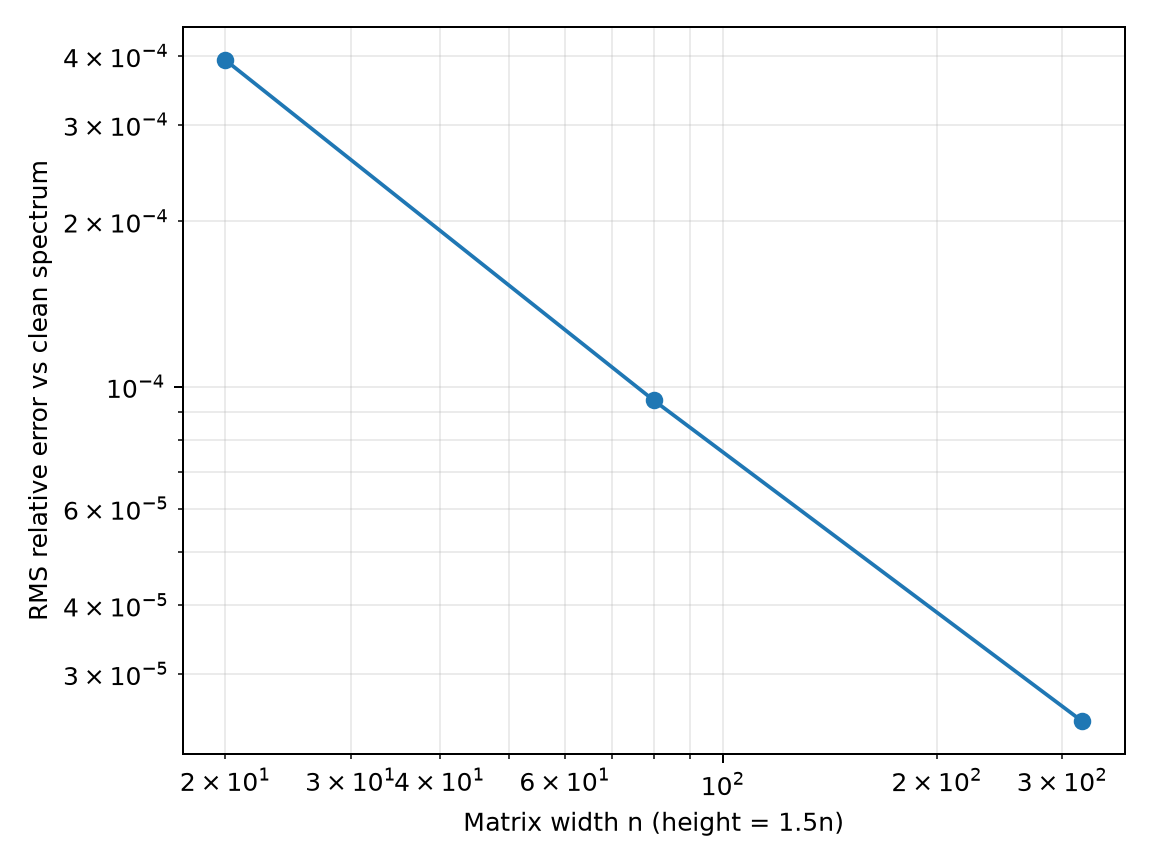
\includegraphics[width=\linewidth]{simulation_error.png}
\end{minipage}\hfill
\begin{minipage}{0.49\linewidth}
\small
\begin{tabular}{@{}lr@{}}\toprule
Size ($m\times n$) & RMS relative error\\\midrule
$30\times20$ & $3.9336608\times10^{-4}$\\
$120\times80$ & $9.4473875\times10^{-5}$\\
$480\times320$ & $2.4609844\times10^{-5}$\\\bottomrule
\end{tabular}\par\medskip
Consecutive ratios (derived): $4.16$ and $3.84$ for each fourfold increase in $n$. No regression slope was fitted.
\end{minipage}
\caption{RMS relative spectral error~\eqref{eq:rms} against width, log--log axes, seeds 0--9 per size. Source: \texttt{outputs/simulation\_error.png} and \texttt{outputs/simulation.txt}.}
\label{fig:sweep}
\end{figure}

This is a dimension sweep, rather than the usual $1/\sqrt n$ consistency experiment for a fixed-parameter sample mean. Equation~\eqref{eq:firstorder} gives a first-order singular-value error SD of $0.01$. For fixed rank, $L^\top L/m$ and $RR^\top/n$ approach identity as dimensions grow, so the nonzero signal singular values grow on the scale $\sqrt{mn}$. Relative errors can therefore decrease on the scale $0.01/\sqrt{mn}\propto1/n$ at fixed aspect ratio. The measured ratios near 4 are consistent with this signal-growth explanation. Three sizes and ten seeds do not establish a precise rate.

\subsection{Stress test: requesting \texorpdfstring{$k=8$}{k=8} from a rank-5 signal}\label{sec:stress}
Requesting $k=8$ forces the solver past the signal into noise components, whose singular values are closely spaced. Table~\ref{tab:stress} lists the library ratio $\sigma_{i+1}/\sigma_i$, its square $\rho_i$ from~\eqref{eq:rate}, and the iteration count.

\begin{table}[H]
\centering\small
\caption{Stress test on the baseline matrix. Source: \texttt{outputs/simulation.txt}. Iteration cap 20000, tolerance $2\times10^{-14}$.}
\label{tab:stress}
\begin{tabular}{@{}c rrrc l@{}}\toprule
$i$ & $\sigma_{i+1}/\sigma_i$ & $\rho_i=(\sigma_{i+1}/\sigma_i)^2$ & Steps & Converged & Regime\\\midrule
1 & 0.919597 & 0.845660 & 174 & yes & signal\\
2 & 0.945341 & 0.893670 & 260 & yes & signal\\
3 & 0.826474 & 0.683060 & 77 & yes & signal\\
4 & 0.916595 & 0.840147 & 172 & yes & signal\\
5 & 0.002642 & 0.000007 & 4 & yes & signal-to-noise gap\\
6 & 0.968960 & 0.938884 & 436 & yes & noise\\
7 & 0.987454 & 0.975065 & 1069 & yes & noise\\
8 & 0.992738 & 0.985529 & 1752 & yes & noise\\\bottomrule
\end{tabular}
\end{table}

All eight components met the stopping rule within the cap. The noise components need 436, 1069 and 1752 steps, versus four across the large signal-to-noise gap. This observed slowdown agrees with the asymptotic rate~\eqref{eq:rate}; exact counts also depend on the random starting vector and stopping rule. Weak separation is the assumption deliberately stressed. A small step change is less informative near a tie: in the linear asymptotic regime, remaining error can be about $\rho/(1-\rho)$ times the last change. The scripts compare components 1--5 with the library but do not separately verify the accuracy of components 6--8.

%======================================================================
\section{Real data: the camera photograph}\label{sec:real}

\subsection{Data and preprocessing}
The input is the same file as Iteration 2: \fn{data/camera.png}, the scikit-image \emph{camera} photograph (Lav Varshney, CC0)~\cite{skimage}. \fn{my\_load\_image} confirms a single-channel 8-bit image of shape $512\times512$ with zero missing values, range $[0,255]$, mean $129.0607$ and PNG file size $139512$ bytes. The only transformation is $A=p/255$ to float64 in $[0,1]$. We remove no pixels and do no resizing, imputation, centering or train/test split; the data matrix is the whole image. Because the image is not centered, the first component largely encodes mean brightness and dominates the energy.

\subsection{Rank selection and reconstructions}
The script starts with $k=50$ power-iteration components and would double $k$ if $95\%$ energy were not reached; $50$ suffice. The energy fraction at rank $k$ is $\sum_{i\le k}\sigma_i^2\big/\sum_{ij}A_{ij}^2$. The first rank reaching $95\%$ is $k_{95}=3$, with $95.09558793\%$ retained, against $92.03269190\%$ at $k=2$. NumPy gives the same $k_{95}$ exactly.

\begin{figure}[H]
\centering
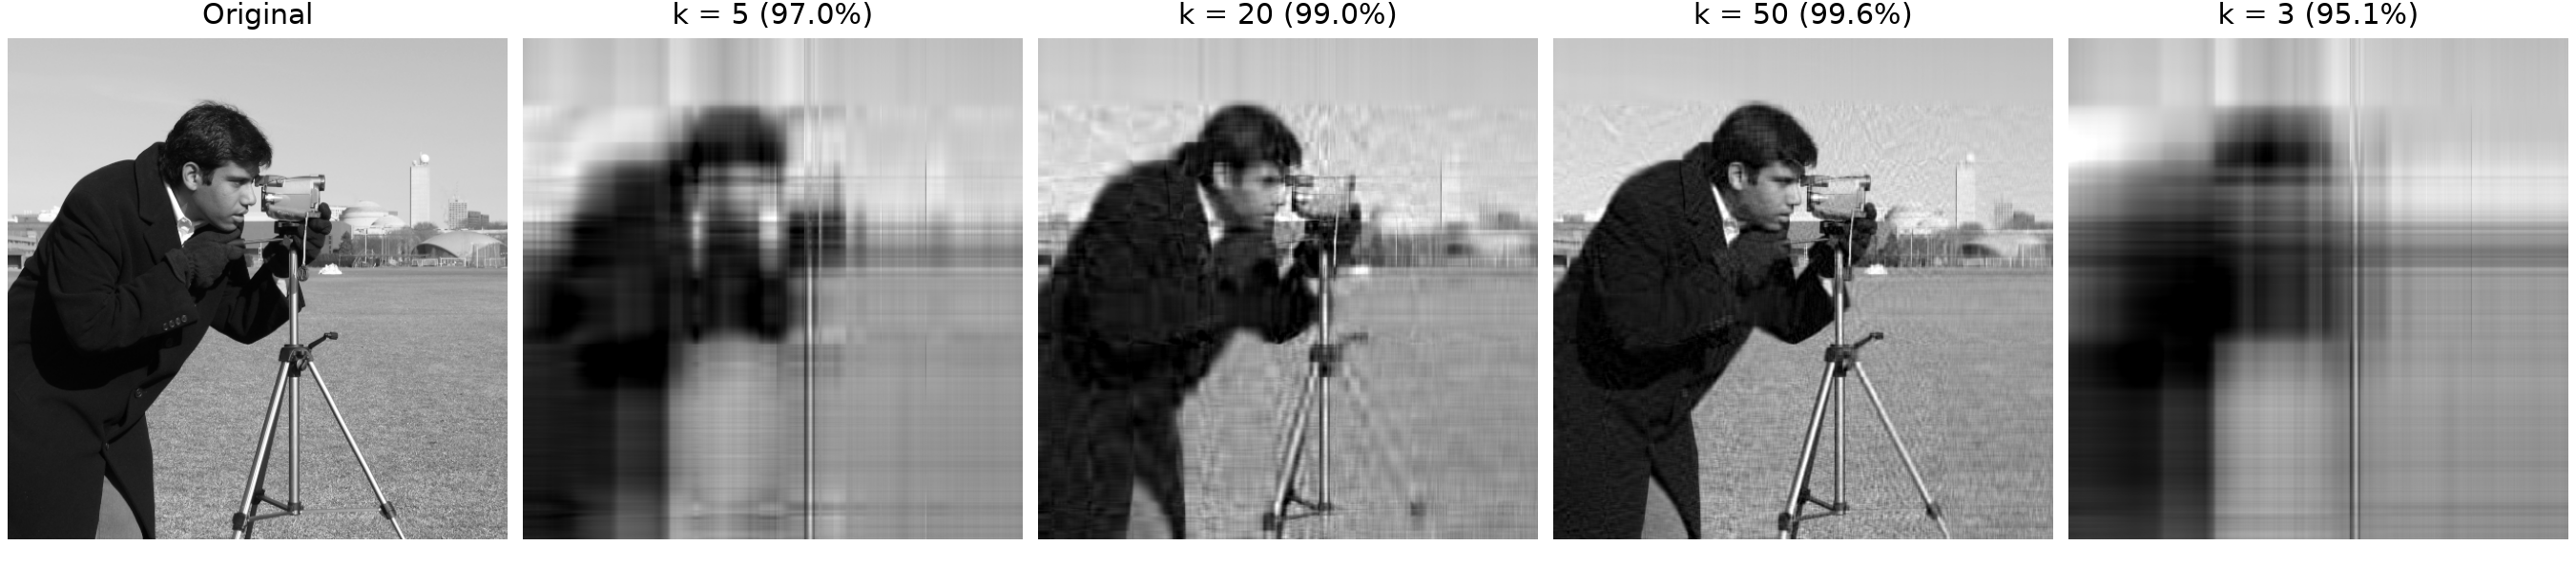
\includegraphics[width=\linewidth]{image_reconstructions.png}
\caption{Original and rank-$k$ reconstructions for $k=5,20,50$ and $k_{95}=3$; titles show the retained energy. Display uses \texttt{imshow} with limits $[0,1]$, which clips out-of-range values for display only. Source: \texttt{outputs/image\_reconstructions.png}.}
\label{fig:recon}
\end{figure}

Figure~\ref{fig:recon} shows that \emph{95\% energy is not perceptual fidelity}. At $k=3$ the image is a set of horizontal and vertical bands, since each term $\sigma_iu_iv_i^\top$ is a separable product of one column profile and one row profile. At $k=5$ a coarse silhouette appears; at $k=20$ the photographer, camera and tripod are recognizable but streaks and ringing remain; at $k=50$ the main structure is clear, while fine grass texture and the distant buildings are softened. The uncentered energy criterion gives substantial weight to broad brightness structure. Squared pixel loss gives no special weight to edges or perceptually important detail.

\begin{figure}[H]
\centering
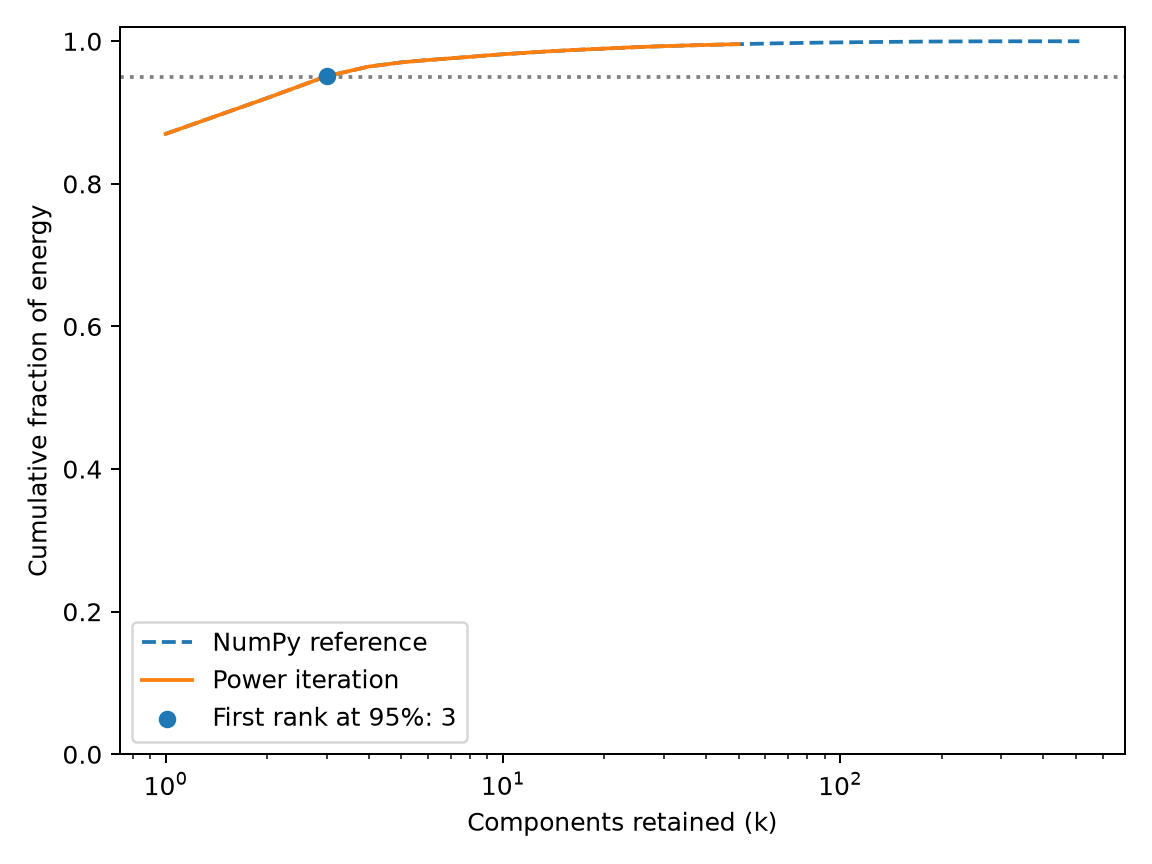
\includegraphics[width=0.62\linewidth]{image_energy.png}
\caption{Cumulative energy fraction against $k$ (log axis). The solid curve covers the 50 components computed by power iteration; the dashed curve uses all 512 NumPy reference values. The dotted line marks 95\%. Source: \texttt{outputs/image\_energy.png}.}
\label{fig:energy}
\end{figure}

\subsection{Error and storage}
\begin{table}[H]
\centering\footnotesize
\caption{Energy, error and storage on the $512\times512$ photograph. Source: \texttt{outputs/real\_image.txt} (stdout of \texttt{src/run\_real.py}). Scalars $=k(m+n+1)$; the share of the $262144$ original entries is derived. Raw factor bytes are float64; the original is $262144$ uint8 bytes and the PNG file is $139512$ bytes. NPZ is measured by \texttt{numpy.savez\_compressed} in memory.}
\label{tab:storage}
\begin{tabular}{@{}r r r r r r r@{}}\toprule
$k$ & Energy & $\|A-A_k\|_F^2$ & Scalars & Share & Raw bytes & NPZ bytes\\\midrule
3 & 95.09558793\% & 4365.6628602 & 3075 & 1.17\% & 24600 & 23951\\
5 & 97.04111655\% & 2633.85038043 & 5125 & 1.96\% & 41000 & 39743\\
20 & 98.97569900\% & 911.781634672 & 20500 & 7.82\% & 164000 & 157592\\
50 & 99.59594419\% & 359.670318826 & 51250 & 19.55\% & 410000 & 393354\\\bottomrule
\end{tabular}
\end{table}

Each squared residual in Table~\ref{tab:storage} is computed from the unclipped, unrounded float64 reconstruction and matches the library tail $\sum_{i>k}\sigma_i^2$; clipping to $[0,1]$ or rounding to 8 bits would break the identity~\eqref{eq:tail}, which is why clipping is applied only when displaying. Counting scalars, truncation saves space whenever $k\le255$. Counting raw bytes, however, each float64 factor entry costs 8 bytes against 1 byte per pixel, so savings require $8k(1025)<262144$, that is $k\le31$; at $k=50$ the raw factors ($410000$ bytes) exceed the original. General-purpose compression barely shrinks float64 factors (e.g.\ $41000\to39743$ bytes at $k=5$). Among the four ranks tested, only $k=3$ and $k=5$ give NPZ files smaller than the $139512$-byte lossless PNG, and those reconstructions are poor. A practical codec would quantize the factors, which we did not test.

%======================================================================
\section{Verification}\label{sec:verify}

\subsection{Comparing singular vectors without sign or basis ambiguity}
Singular vectors are not unique: $(u_i,v_i)$ and $(-u_i,-v_i)$ are equally valid, and inside a repeated singular value any common rotation of the paired bases is valid. \fn{compare\_svd} therefore does \emph{not} compare sign-aligned vectors directly. It groups the reference singular values into blocks $[s,e)$ whose members differ by at most $64\,\eps\max(m,n)\,\sigma_1^{\text{ref}}$; for the retained columns $[s,t)$ with $t=\min(e,k)$ it forms the coefficient matrix and residuals
\begin{equation}\label{eq:subspace}
C=\big(V^{\text{ref}}_{[s,e)}\big)^{\!\top}V_{[s,t)},\qquad
R_V=V_{[s,t)}-V^{\text{ref}}_{[s,e)}C,\qquad
R_U=U_{[s,t)}-U^{\text{ref}}_{[s,e)}C,
\end{equation}
and requires $\max|R_V|,\max|R_U|\le10^{-8}$. $R_V$ is the residual after projecting the computed right vectors onto the reference right singular subspace. $R_U$ applies the \emph{same} coefficients to the left vectors, so it checks that left and right vectors are correctly paired. For a singleton block, $C$ is a $1\times1$ overlap close to $\pm1$, so a common sign flip of $(u_i,v_i)$ passes but flipping only $u_i$ fails. For a fully retained repeated block, $C$ is nearly orthogonal. When $k$ cuts through the block, $C$ is rectangular with approximately orthonormal columns ($C^\top C\approx I$). Both cases allow a common change of basis while preserving the left/right pairing. In both experiments every block was a singleton (labels $i{:}i$ in the outputs). Seven regression tests in \fn{tests/test\_verification.py} exercise these cases: sign flips and rotated or partially retained tied blocks must pass; inconsistent left/right rotations, rotations across distinct values, wrong spectra, non-orthonormal factors, NaN/Inf values and assumption failures must exit with an error.

\subsection{Verification table}
A check passes when $\max|\text{diff}|\le\texttt{atol}+\texttt{rtol}\cdot\max|\text{ref}|$; failure stops the script with a nonzero exit code. Unless stated otherwise $\texttt{atol}=10^{-8}$ and $\texttt{rtol}=0$.

\begin{table}[H]
\centering\small
\caption{Summary of verification checks on the committed outputs. Each listed comparison passed its script's rule. Maxima across vector blocks are labelled as aggregates; complete stdout and the independent rerun are retained in the repository.}
\label{tab:verify}
\begin{tabularx}{\linewidth}{@{}P{1.75cm} L P{2.4cm} P{2.2cm} c@{}}\toprule
Data & Quantity and reference & Difference & Pass rule & Pass?\\\midrule
Small & $A_1$ vs exact fractions & $8.882\times10^{-16}$ & max $\le10^{-8}$ & Yes\\
Small & Squared error vs exact $5$ & $0$ & max $\le10^{-8}$ & Yes\\
Small & $GV$ vs $V\Sigma^2$ & $7.105\times10^{-15}$ & max $\le10^{-8}$ & Yes\\
Small & Power spectrum vs exact values & $4.441\times10^{-16}$ & max $\le10^{-8}$ & Yes\\\midrule
Simulation & Top 5 values vs clean truth & $1.862\times10^{-2}$ & max $\le0.03$ & Yes\\
Simulation & Top 5 values vs NumPy SVD & $7.105\times10^{-14}$ & max $\le10^{-8}$ & Yes\\
Simulation & $R_V$; $R_U$ (max over 5 blocks) & $1.629\times10^{-13}$; $1.752\times10^{-13}$ & each max $\le10^{-8}$ & Yes\\
Simulation & Squared residual vs library tail & $1.776\times10^{-15}$ & max $\le10^{-8}+10^{-12}|\mathrm{tail}|$ & Yes\\
Stress & Stopping criterion, $k=8$ & 8 of 8 converged & cap 20000 steps & Yes\\\midrule
Image & $k_{95}$ vs NumPy & $0$ & exact equality & Yes\\
Image & 50 values vs NumPy SVD & $3.553\times10^{-14}$ & max $\le10^{-8}$ & Yes\\
Image & $R_V$; $R_U$ (max over 50 blocks) & $1.892\times10^{-12}$; $1.830\times10^{-12}$ & each max $\le10^{-8}$ & Yes\\
Image & Squared error vs tail, $k=3,5,20,50$ & $2.728\times10^{-12}$ (largest) & each max $\le10^{-8}$ & Yes\\\midrule
Tests & Existing regression tests (fresh run) & 7 of 7 passed & expected assertions & Yes\\\bottomrule
\end{tabularx}
\end{table}


The library tolerance $10^{-8}$ is loose compared with the observed $10^{-16}$--$10^{-12}$ discrepancies, so it detects real errors without flagging roundoff. The truth tolerance $0.03$ measures statistical error, not roundoff, and is justified by~\eqref{eq:firstorder}.

%======================================================================
\section{Assumptions and their checks}\label{sec:assump}
Table~\ref{tab:assump} lists each assumption the method relies on, what goes wrong if it fails, and the measured check, simulation first and then the photograph.

\begin{table}[H]
\centering\footnotesize
\caption{Assumption checks from \texttt{check\_assumptions} and the data loader. Sources: \texttt{outputs/simulation.txt}, \texttt{outputs/real\_image.txt}.}
\label{tab:assump}
\begin{tabularx}{\linewidth}{@{}P{2.5cm} P{3.1cm} L L@{}}\toprule
Assumption & If violated & Simulation ($120\times80$, $k=5$) & Photograph ($512\times512$, $k=50$)\\\midrule
Complete finite real 2-D grid & Gram product undefined; color tuples are not scalars & shape $(120,80)$, finite $9600/9600$, float64, range $[-11.0534,11.7929]$ & 1 channel uint8, missing 0; finite $262144/262144$ float64, range $[0,1]$\\
Gram symmetric PSD~\eqref{eq:psd} & $\sqrt{\lambda_i}$ undefined & $\max|G-G^\top|=0$; $\lambda_{\min}=4.8961674\times10^{-4}\ge-\tau$ & $0$; $\lambda_{\min}=5.5171395\times10^{-10}\ge-\tau$\\
Retained values above cutoff~\eqref{eq:cutoff} & Division by $\approx0$ in $U=AV\Sigma^{-1}$ & $\tau=3.1745165\times10^{-10}$; smallest retained $\lambda=5167.054$ & $\tau=8.8050313\times10^{-9}$; smallest retained $\lambda=8.8182777$\\
Factor orthogonality~\eqref{eq:uorth} & Cross terms break~\eqref{eq:frobinner} & $6.322\times10^{-14}$ ($U$), $2.220\times10^{-16}$ ($V$) & $1.643\times10^{-13}$ ($U$), $5.551\times10^{-16}$ ($V$)\\
Descending order & ``First $k$'' is not the best $k$ & true & true\\
Spectral separation & Slow power iteration; truth band~\eqref{eq:firstorder} invalid & signal gap $\sigma_6/\sigma_5=0.002642$; noise ratios up to $0.992738$ (Table~\ref{tab:stress}) & no numerical ties at the reference tolerance; this alone does not show wide gaps. The $k=50$ solver and orthogonality checks passed\\
Squared, unweighted loss~\eqref{eq:tail} & Tail no longer predicts error & residual $=$ tail $=0.873022217597$ & residual $=$ tail $=359.670318826$; unclipped float64\\
Noise model (truth band only) & $0.03$ band uncalibrated & i.i.d.\ $N(0,0.01^2)$ by construction & not applicable: no ground truth\\
Storage precision & Scalar count misstates bytes & $1005/9600$ scalars; $8040/76800$ bytes (float64 both) & $51250/262144$ scalars; $410000/262144$ bytes (float64 factors vs uint8 pixels)\\\bottomrule
\end{tabularx}
\end{table}

On the photograph the smallest library Gram eigenvalue ($5.5\times10^{-10}$) lies below $\tau=8.8\times10^{-9}$, so a full-rank run would stop before that component. This has no effect on $k\le50$, where the smallest retained eigenvalue is $8.82$.

%======================================================================
\section{Discussion and limitations}\label{sec:discuss}
\begin{itemize}[leftmargin=1.2em]
\item \textbf{Squared conditioning and cutoff.} On the positive singular subspace, $\kappa_2(A^\top A)=\kappa_2(A)^2$. Forming the Gram matrix loses relative accuracy for small singular values~\cite{trefethen1997,golub2013}. The cutoff~\eqref{eq:cutoff} excludes sufficiently small components; it suits this leading-component approximation but does not produce a complete, accurate tiny spectrum.
\item \textbf{The cutoff} $\tau$ is a roundoff heuristic, not a statistical threshold. It does not separate signal from noise; in the simulation, the large gap after $\sigma_5$ does that.
\item \textbf{Slow convergence for close spectra.} By~\eqref{eq:rate} the cost grows like $1/\log(1/\rho_i)$. Near-ties (noise components, or textured images) raise step counts sharply, and a fixed step tolerance certifies less when $\rho_i\to1$. Block or Lanczos methods would be the next step.
\item \textbf{Scope of evidence.} The real-data results come from one image, so the energy and storage figures do not generalize to other images. The size sweep uses ten seeds at three sizes, enough to show the trend but not to estimate a rate or its uncertainty. The $0.03$ band rests on a first-order, per-value approximation.
\item \textbf{Energy is not quality.} Uncentered energy fractions are inflated by mean brightness; $95\%$ energy at $k=3$ is visually poor. A perceptual metric was out of scope.
\end{itemize}

%======================================================================
\section{Team, leadership and review record}\label{sec:team}

\textbf{Project lead.} Jiaxiao Chen leads Iteration 3; Jiaxiao also led Iteration 1, and Alexander Rees led Iteration 2. The handout asks each iteration to have a leader who has not previously led. With two members and three iterations that rule cannot be met, so the team needs an instructor exception; it is \emph{pending} and is not claimed here.

\textbf{Contributions.} The team reports an equal overall contribution split: Jiaxiao Chen 50\% and Alexander Rees 50\%, confirmed by the user on November 22, 2026. The Iteration 3 implementation and stored outputs are recorded in commit \fn{3a7dc93}. No task-by-task allocation is inferred from commit authorship.

\textbf{AI assistance.} At the user's request, this report was drafted with Claude assistance and independently reviewed with Codex against the handout, source code, committed outputs and fresh script runs. That review is recorded separately. It is not a student signature and does not replace the required check by the second team member.

\begin{table}[H]
\centering\small
\caption{Overall contributions, as confirmed by the user.}
\label{tab:contrib}
\begin{tabularx}{\linewidth}{@{}L r L@{}}\toprule
Member & Overall share & Confirmation\\\midrule
Jiaxiao Chen & 50\% & Equal contribution, user-confirmed\\
Alexander Rees & 50\% & Equal contribution, user-confirmed\\\bottomrule
\end{tabularx}
\end{table}
\textbf{Technical review.} The report presents a clear mathematical derivation and consistently connects the equations to the shared implementation. The exact example, reproducible simulation and real-image experiments give strong support for the leading-component results. All three scripts and all seven existing verification tests passed. The assumptions, storage trade-offs and numerical limitations are explained clearly. This positive assessment records the completed AI-assisted technical review; student peer-check details can be recorded separately in the project plan.

\section{Reproducibility}\label{sec:repro}
\textbf{Independent rerun.} On November 22, 2026, all three unchanged scripts and all seven existing regression tests passed using Python 3.12.14, NumPy 2.5.5, Matplotlib 3.11.2 and Pillow 13.0.0 on macOS ARM64. Fresh stdout and source checksums are retained in \fn{docs/verification-2026-11-22/}. The fresh simulation value comparison gives $4.263\times10^{-14}$ instead of the committed $7.105\times10^{-14}$; the image's largest per-rank tail discrepancy is $3.638\times10^{-12}$ instead of $2.728\times10^{-12}$. Both remain below $10^{-8}$. Measured NPZ byte counts also vary slightly with floating-point factor entries and serialization. The three regenerated PNGs are byte-identical to the committed figures. Table~\ref{tab:verify} consistently cites the committed run except for its explicitly labelled fresh test row.


From the repository root, with the packages in \fn{requirements.txt} (NumPy, Matplotlib, Pillow) installed:
\begin{center}\small
\begin{tabular}{@{}l l@{}}\toprule
Command & Stored output and report location\\\midrule
\fn{python src/small\_example.py} & \fn{outputs/small\_example.txt}; Sec.~\ref{sec:small}, Table~\ref{tab:small}\\
\fn{python src/check\_simulation.py} & \fn{outputs/simulation.txt}, \fn{simulation\_error.png}; Sec.~\ref{sec:sim}\\
\fn{python src/run\_real.py} & \fn{outputs/real\_image.txt}, \fn{image\_*.png}; Sec.~\ref{sec:real}\\
\fn{python -m unittest discover -s tests -v} & regression tests; Sec.~\ref{sec:verify}\\\bottomrule
\end{tabular}
\end{center}
\clearpage
\begin{thebibliography}{9}\small
\bibitem{eckart1936} C.~Eckart and G.~Young, ``The approximation of one matrix by another of lower rank,'' \emph{Psychometrika} 1(3):211--218, 1936.
\bibitem{golub2013} G.~H.~Golub and C.~F.~Van~Loan, \emph{Matrix Computations}, 4th ed., Johns Hopkins University Press, 2013.
\bibitem{trefethen1997} L.~N.~Trefethen and D.~Bau~III, \emph{Numerical Linear Algebra}, SIAM, 1997.
\bibitem{skimage} scikit-image 0.25.2 documentation, \href{https://scikit-image.org/docs/0.25.x/api/skimage.data.html\#skimage.data.camera}{\emph{camera} dataset}. Photograph by Lav Varshney, CC0. Accessed November 22, 2026.
\bibitem{numpy} NumPy documentation, \href{https://numpy.org/doc/stable/reference/generated/numpy.linalg.svd.html}{\fn{numpy.linalg.svd}}. Reference factorization and return conventions. Accessed November 22, 2026.
\end{thebibliography}

\end{document}
